\documentclass{article}
\usepackage[utf8]{inputenc}
\usepackage{geometry}
\usepackage{graphicx}
\usepackage{float}
\usepackage{enumitem}  % Added package for customizing itemize spacing

\geometry{a4paper, total={5.5in, 7.5in}, left=0.75in, right=0.75in, top=0.75in, bottom=0.75in}

\title{Database Design Report}
\author{Ioannis Zacharopoulos (2307)/Dimitrios Tselentis (2325)}
\begin{document}

\maketitle

\section*{\centering Database Design Explanation}


\subsection*{Roles Table}
The \texttt{roles\_2307\_2325} table holds distinct roles (e.g., protector, beneficiary, shareholder, director). This table provides a centralized location to manage roles, allowing for flexibility in adding new roles without altering the overall database schema. Each role is uniquely identified by a \texttt{role\_id} and includes a \texttt{role\_type} field to specify the role, a role may be between an officer to entity, an officer to officer and a officer to intermediary.

\subsection*{Entities Table}
The \texttt{entities\_2307\_2325} table represents offshore entities. Each entity has a unique identifier (\texttt{entity\_id}), and its details, such as name, jurisdiction, country code, incorporation date, etc., are stored in this table. This table serves as the core repository for entity information, allowing for efficient retrieval and management of offshore entities.

\subsection*{Officers Table}
The \texttt{officers\_2307\_2325} table contains information about officers associated with entities. Officers may include individuals holding positions like directors, shareholders etc. This table includes details such as name, country code, and other relevant information about officers.

\subsection*{Officers\_Roles\_Entities Table}
The \texttt{officers\_roles\_entities\_2307\_2325} table represents the many-to-many relationship between officers, roles, and entities. It captures information about an officer's role in a specific entity. This structure allows for the representation of complex relationships between officers, roles, and entities.

\subsection*{Officers\_Roles\_Officers Table}
The \texttt{officers\_roles\_officers\_2307\_2325} table represents another many-to-many relationship, specifically for relationships between officers. It captures information about the relationships between two officers and their roles.

\subsection*{Officers\_Roles\_Intermediaries Table}
The \texttt{officers\_roles\_intermediaries\_2307\_2325} table represents the many-to-many relationship between officers, roles, and intermediaries. It captures information about an officer's role in relation to an intermediary.

\subsection*{Intermediaries Table}
The \texttt{intermediaries\_2307\_2325} table contains information about intermediaries associated with entities. Intermediaries may include legal entities or individuals providing services. This table includes details such as name, country code, status, etc.

\subsection*{Addresses Table}
The \texttt{addresses\_2307\_2325} table stores address information that can be associated with officers or entities. It includes details such as the name, address, country code, etc.

\subsection*{Intermediaries\_Entities Table}
The \texttt{intermediaries\_entities\_2307\_2325} table represents the many-to-many relationship between intermediaries and entities. It captures information about the association between an intermediary and an entity.

\subsection*{Officers\_Addresses Table}
The \texttt{officers\_addresses\_2325} table represents the many-to-many relationship between officers and addresses. It captures information about an officer's association with an address.

\subsection*{Entities\_Addresses Table}
The \texttt{entities\_addresses\_2325} table represents the many-to-many relationship between entities and addresses. It captures information about an entity's association with an address.


\section*{\centering Database Relations}


\begin{minipage}{0.5\textwidth}

    \subsubsection*{Roles Table}
    \texttt{roles\_2307\_2325}:
    \begin{itemize}
        \item \texttt{role\_id} (PK)
        \item \texttt{role\_type}
    \end{itemize}

    \subsubsection*{Entities Table}
    \texttt{entities\_2307\_2325}:
    \begin{itemize}
        \item \texttt{entity\_id} (PK)
        \item \texttt{name}
        \item \texttt{jurisdiction}
        \item \texttt{jurisdiction\_description}
              % (Other attributes truncated for brevity)
    \end{itemize}

    \subsubsection*{Officers Table}
    \texttt{officers\_2307\_2325}:
    \begin{itemize}
        \item \texttt{officer\_id} (PK)
        \item \texttt{name}
              % (Other attributes truncated for brevity)
    \end{itemize}

    \subsubsection*{Officers\_Roles\_Entities Table}
    \texttt{officers\_roles\_entities\_2307\_2325}:
    \begin{itemize}
        \item \texttt{officer\_role\_entity\_id} (PK)
        \item \texttt{officer\_id} (FK)
        \item \texttt{role\_id} (FK)
        \item \texttt{entity\_id} (FK)
              % (Other attributes truncated for brevity)
    \end{itemize}

    \subsubsection*{Officers\_Roles\_Officers Table}
    \texttt{officers\_roles\_officers\_2307\_2325}:
    \begin{itemize}
        \item \texttt{officer\_role\_officer\_id} (PK)
        \item \texttt{officer\_id\_1} (FK)
        \item \texttt{role\_id} (FK)
        \item \texttt{officer\_id\_2} (FK)
              % (Other attributes truncated for brevity)
    \end{itemize}

\end{minipage}
\hspace{0.05\textwidth}
\begin{minipage}{0.5\textwidth}

    \subsubsection*{Officers\_Roles\_Intermediaries Table}
    \texttt{officers\_roles\_intermediaries\_2307\_2325}:
    \begin{itemize}
        \item \texttt{officer\_role\_intermediary\_id} (PK)
        \item \texttt{officer\_id} (FK)
        \item \texttt{role\_id} (FK)
        \item \texttt{intermediary\_id} (FK)
              % (Other attributes truncated for brevity)
    \end{itemize}

    \subsubsection*{Intermediaries Table}
    \texttt{intermediaries\_2307\_2325}:
    \begin{itemize}
        \item \texttt{intermediary\_id} (PK)
        \item \texttt{name}
              % (Other attributes truncated for brevity)
    \end{itemize}

    \subsubsection*{Addresses Table}
    \texttt{addresses\_2307\_2325}:
    \begin{itemize}
        \item \texttt{address\_id} (PK)
        \item \texttt{name}
              % (Other attributes truncated for brevity)
    \end{itemize}

    \subsubsection*{Intermediaries\_Entities Table}
    \texttt{intermediaries\_entities\_2307\_2325}:
    \begin{itemize}
        \item \texttt{intermediary\_entity\_id} (PK)
        \item \texttt{intermediary\_id} (FK)
        \item \texttt{entity\_id} (FK)
              % (Other attributes truncated for brevity)
    \end{itemize}

    \subsubsection*{Officers\_Addresses Table}
    \texttt{officers\_addresses\_2325}:
    \begin{itemize}
        \item \texttt{officer\_address\_id} (PK)
        \item \texttt{officer\_id} (FK)
        \item \texttt{address\_id} (FK)
              % (Other attributes truncated for brevity)
    \end{itemize}

    \subsubsection*{Entities\_Addresses Table}
    \texttt{entities\_addresses\_2325}:
    \begin{itemize}
        \item \texttt{entity\_address\_id} (PK)
        \item \texttt{entity\_id} (FK)
        \item \texttt{address\_id} (FK)
              % (Other attributes truncated for brevity)
    \end{itemize}

\end{minipage}


\section*{\centering Additional Notes}
There are many more attributes in the tables that are not shown in the above relations. The attributes shown are the ones that are relevant to the queries that we will be executing. The rest of the attributes are not shown for brevity. Additional information about the intuitions behind the design of the database can be found in the \texttt{report2.pdf} file of the project.





\begin{figure}[h]
    \centering
    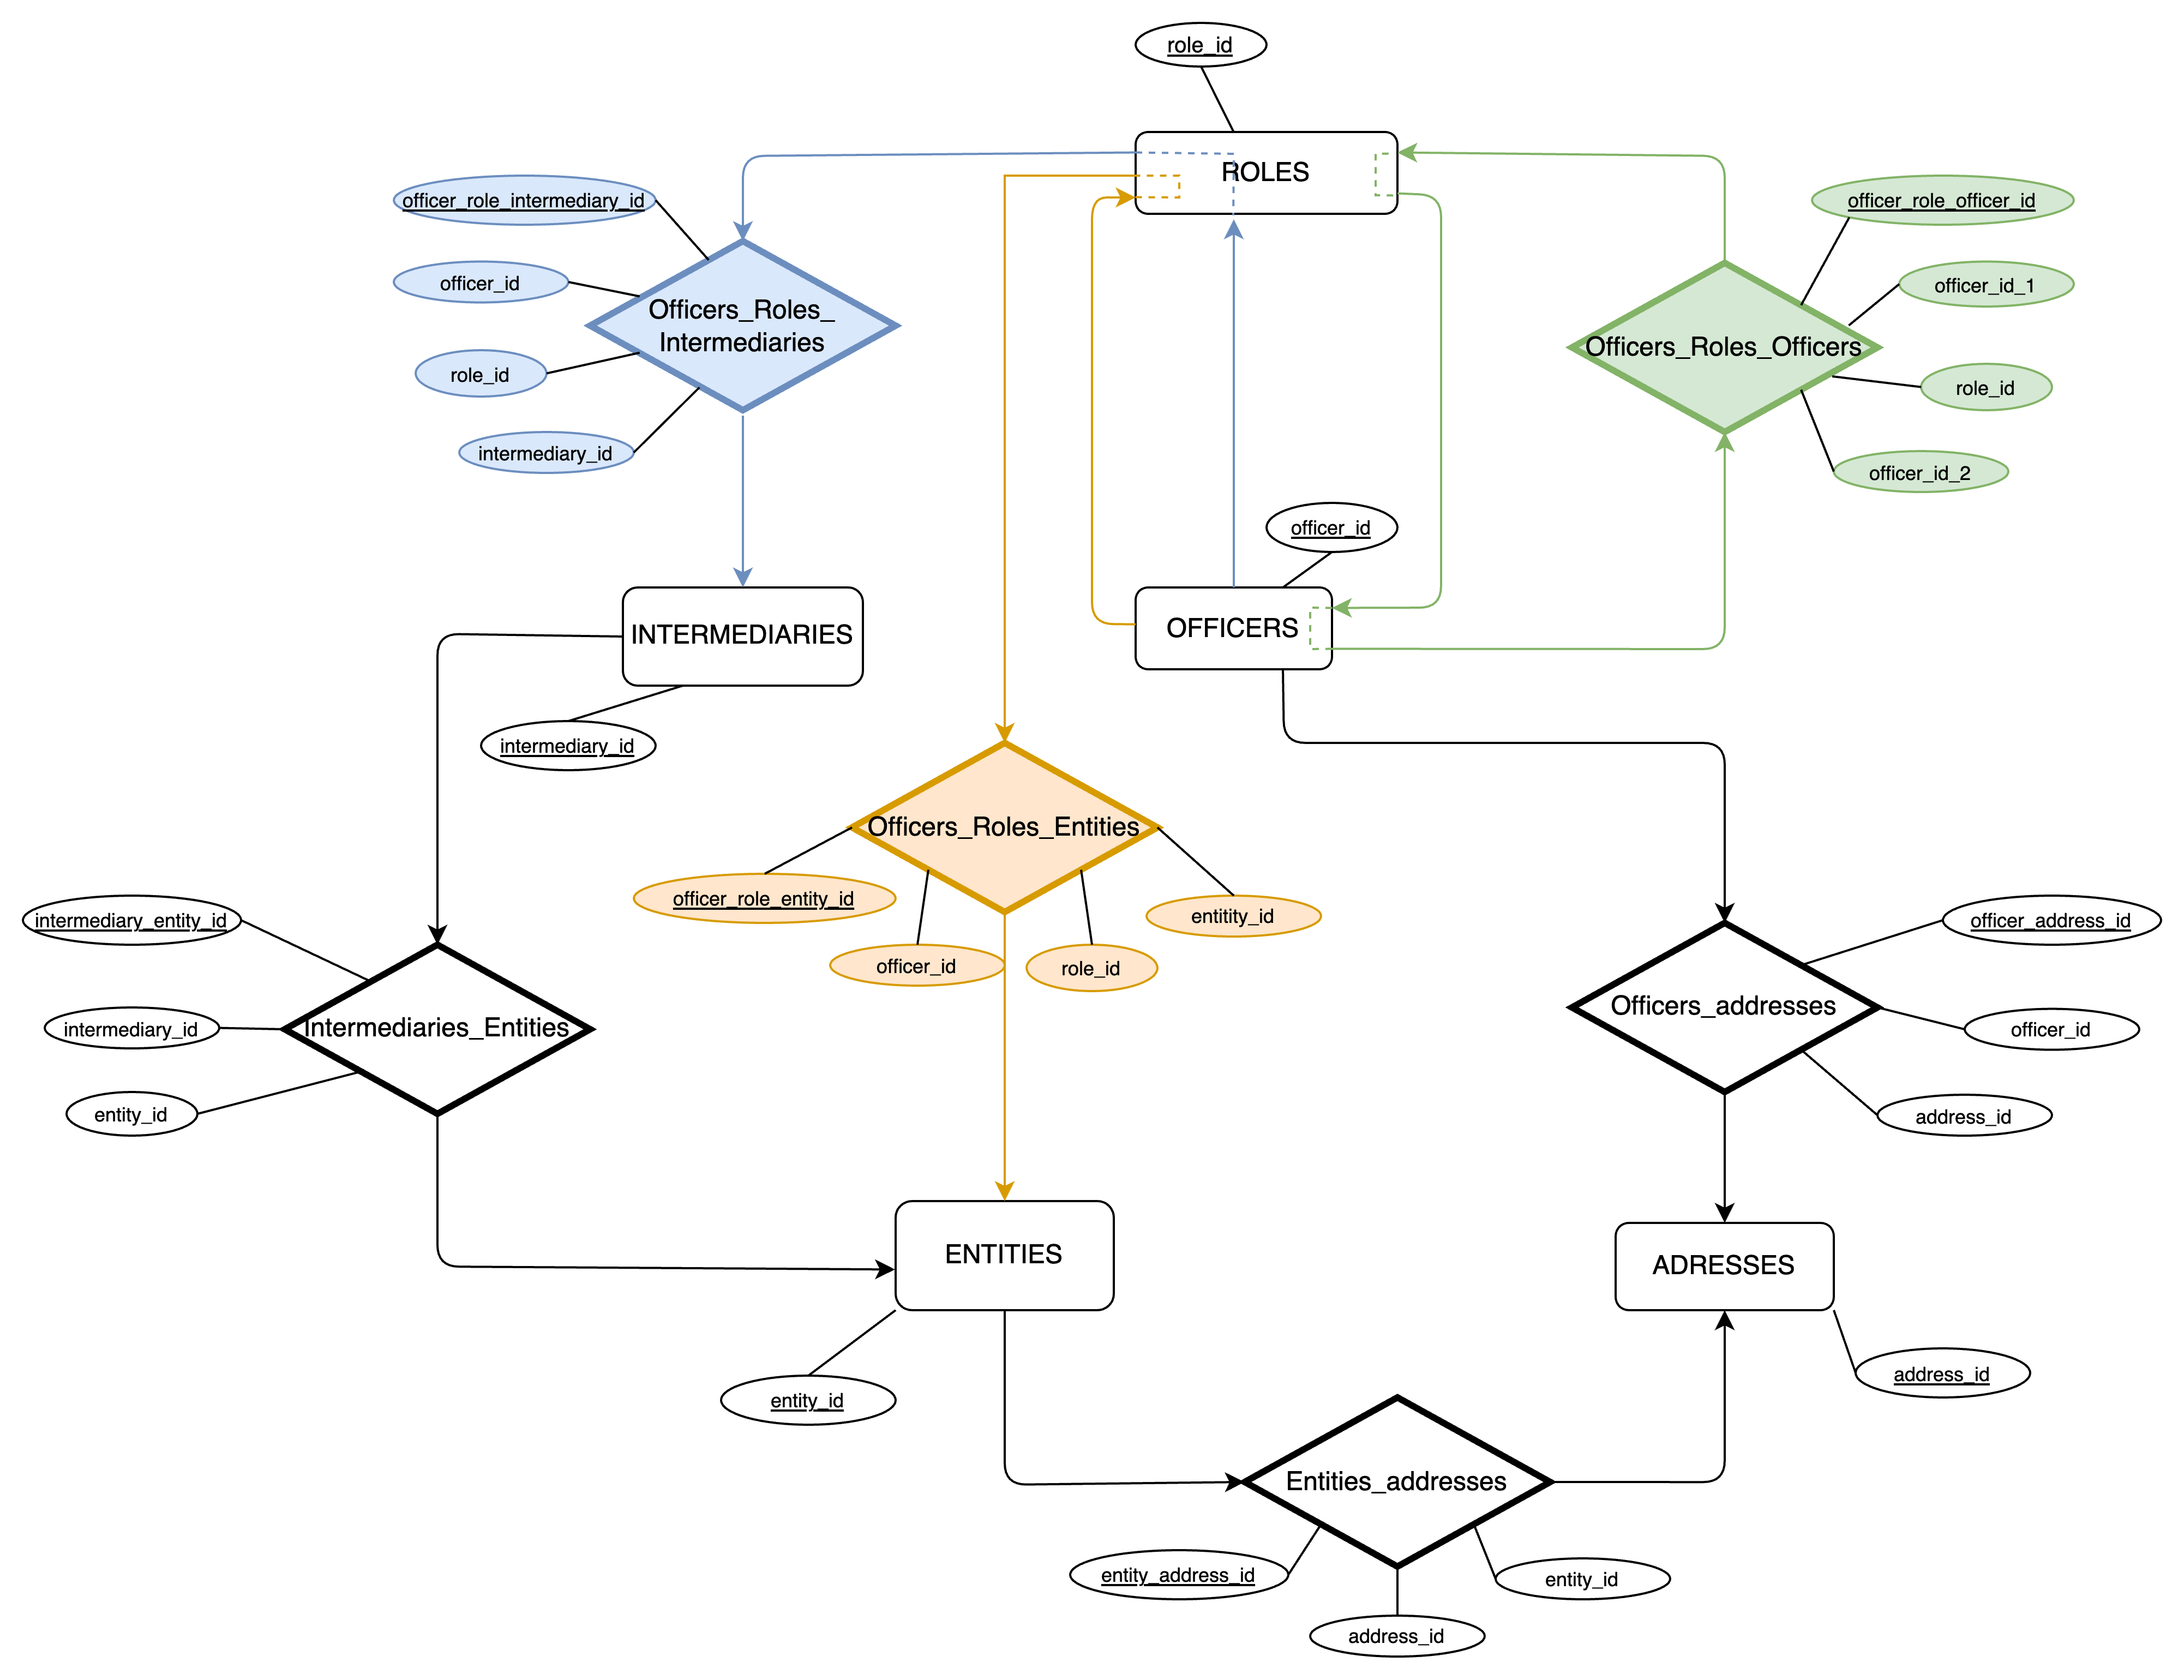
\includegraphics[width=\textwidth]{er.png}
    \caption{ER Diagram}
    \label{fig:er-diagram}
\end{figure}


\end{document}
